

\tikzset{every picture/.style={line width=0.75pt}} %set default line width to 0.75pt        

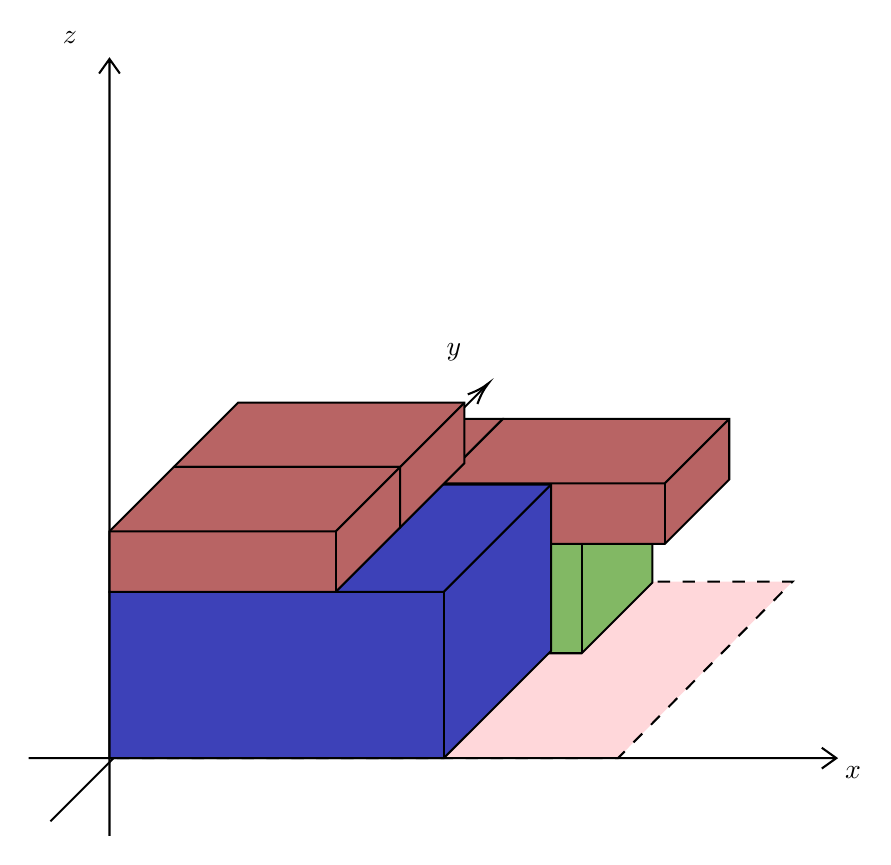
\begin{tikzpicture}[x=0.75pt,y=0.75pt,yscale=-1,xscale=1]
%uncomment if require: \path (0,441); %set diagram left start at 0, and has height of 441

%Shape: Parallelogram [id:dp6336164728589061] 
\draw  [fill={rgb, 255:red, 255; green, 17; blue, 34 }  ,fill opacity=0.17 ][dash pattern={on 4.5pt off 4.5pt}] (261,308.5) -- (506,308.5) -- (421.91,393.57) -- (176.91,393.57) -- cycle ;
%Shape: Axis 2D [id:dp545790083210709] 
\draw  (138,393.57) -- (527.11,393.57)(176.91,56.72) -- (176.91,431) (520.11,388.57) -- (527.11,393.57) -- (520.11,398.57) (171.91,63.72) -- (176.91,56.72) -- (181.91,63.72)  ;
%Straight Lines [id:da23076777818637972] 
\draw    (148.47,424.02) -- (358.19,214.3) ;
\draw [shift={(359.6,212.89)}, rotate = 135] [color={rgb, 255:red, 0; green, 0; blue, 0 }  ][line width=0.75]    (10.93,-3.29) .. controls (6.95,-1.4) and (3.31,-0.3) .. (0,0) .. controls (3.31,0.3) and (6.95,1.4) .. (10.93,3.29)   ;
%Shape: Cube [id:dp6994519250263277] 
\draw  [fill={rgb, 255:red, 130; green, 184; blue, 100 }  ,fill opacity=1 ] (226.47,290.32) -- (260.48,256.32) -- (349.46,256.32) -- (349.46,309.03) -- (315.46,343.04) -- (226.47,343.04) -- cycle ; \draw   (349.46,256.32) -- (315.46,290.32) -- (226.47,290.32) ; \draw   (315.46,290.32) -- (315.46,343.04) ;
%Shape: Cube [id:dp07364374934794116] 
\draw  [fill={rgb, 255:red, 130; green, 184; blue, 100 }  ,fill opacity=1 ] (315.46,290.32) -- (349.46,256.32) -- (438.45,256.32) -- (438.45,309.03) -- (404.44,343.04) -- (315.46,343.04) -- cycle ; \draw   (438.45,256.32) -- (404.44,290.32) -- (315.46,290.32) ; \draw   (404.44,290.32) -- (404.44,343.04) ;
%Shape: Cube [id:dp8273351088299524] 
\draw  [fill={rgb, 255:red, 184; green, 100; blue, 100 }  ,fill opacity=1 ] (226.47,261.16) -- (257.47,230.16) -- (366.49,230.16) -- (366.49,259.32) -- (335.49,290.32) -- (226.47,290.32) -- cycle ; \draw   (366.49,230.16) -- (335.49,261.16) -- (226.47,261.16) ; \draw   (335.49,261.16) -- (335.49,290.32) ;
%Shape: Cube [id:dp12028810160505032] 
\draw  [fill={rgb, 255:red, 184; green, 100; blue, 100 }  ,fill opacity=1 ] (335.49,261.16) -- (366.49,230.16) -- (475.51,230.16) -- (475.51,259.32) -- (444.51,290.32) -- (335.49,290.32) -- cycle ; \draw   (475.51,230.16) -- (444.51,261.16) -- (335.49,261.16) ; \draw   (444.51,261.16) -- (444.51,290.32) ;
%Shape: Cube [id:dp015004623257364513] 
\draw  [fill={rgb, 255:red, 61; green, 65; blue, 184 }  ,fill opacity=1 ] (176.91,313.44) -- (228.61,261.75) -- (389.7,261.75) -- (389.7,341.88) -- (338,393.57) -- (176.91,393.57) -- cycle ; \draw   (389.7,261.75) -- (338,313.44) -- (176.91,313.44) ; \draw   (338,313.44) -- (338,393.57) ;
%Shape: Cube [id:dp6659863306674686] 
\draw  [fill={rgb, 255:red, 184; green, 100; blue, 100 }  ,fill opacity=1 ] (207.91,253.28) -- (238.91,222.28) -- (347.93,222.28) -- (347.93,251.44) -- (316.93,282.44) -- (207.91,282.44) -- cycle ; \draw   (347.93,222.28) -- (316.93,253.28) -- (207.91,253.28) ; \draw   (316.93,253.28) -- (316.93,282.44) ;
%Shape: Cube [id:dp7671953057902039] 
\draw  [fill={rgb, 255:red, 184; green, 100; blue, 100 }  ,fill opacity=1 ] (176.91,284.28) -- (207.91,253.28) -- (316.93,253.28) -- (316.93,282.44) -- (285.93,313.44) -- (176.91,313.44) -- cycle ; \draw   (316.93,253.28) -- (285.93,284.28) -- (176.91,284.28) ; \draw   (285.93,284.28) -- (285.93,313.44) ;

% Text Node
\draw (337.9,192.2) node [anchor=north west][inner sep=0.75pt]    {$y$};
% Text Node
\draw (529.84,396.35) node [anchor=north west][inner sep=0.75pt]    {$x$};
% Text Node
\draw (152.94,42.14) node [anchor=north west][inner sep=0.75pt]    {$z$};


\end{tikzpicture}
